%\setchapterimage{fig_00.jpg}
\chapter*{Application \arabic{cptApplication} \\ 
Stabilité des systèmes -- \ifprof Corrigé \else Sujet \fi}
\addcontentsline{toc}{section}{Application \arabic{cptApplication} : Stabilité des systèmes  -- \ifprof Corrigé \else Sujet \fi}

\iflivret \stepcounter{cptApplication} \else
\ifprof  \stepcounter{cptApplication} \else \fi
\fi

\setcounter{question}{0}
%\marginnote{Concours Centrale -- MP 2019}
\marginnote{
\UPSTIcompetence[2]{C1-01}
\UPSTIcompetence[2]{C2-03}}


\question{On donne ci-dessous les lieux de transferts de plusieurs  FTBO. Déterminer, à l’aide du critère du Revers si les systèmes sont stables en BF. Pour les systèmes stables déterminer les marges de gain et de phase.}
 
\ifprof

\begin{center}
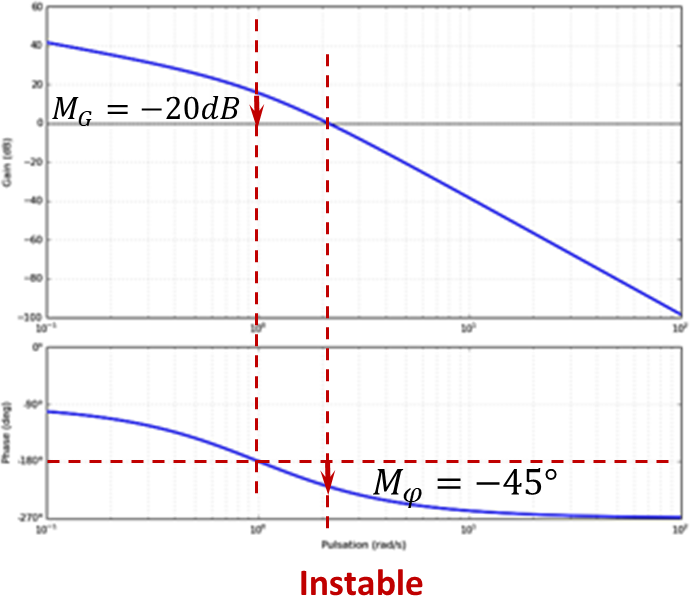
\includegraphics[width=8cm]{im_01_cor}
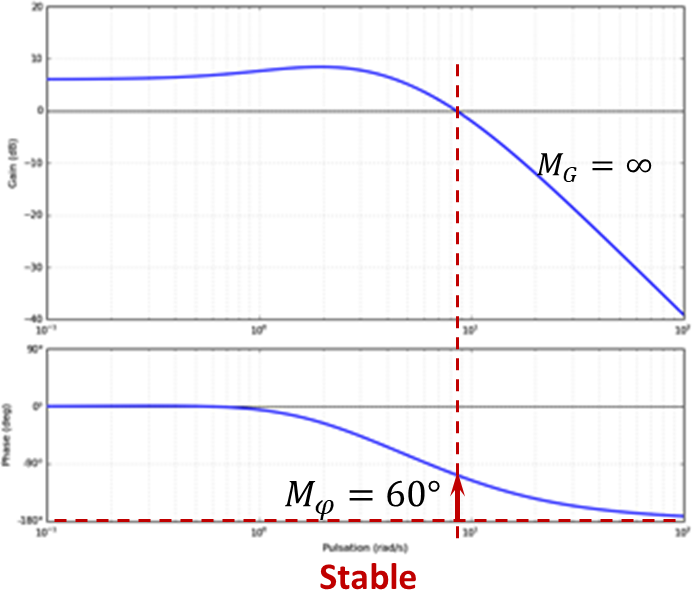
\includegraphics[width=8cm]{im_02_cor}
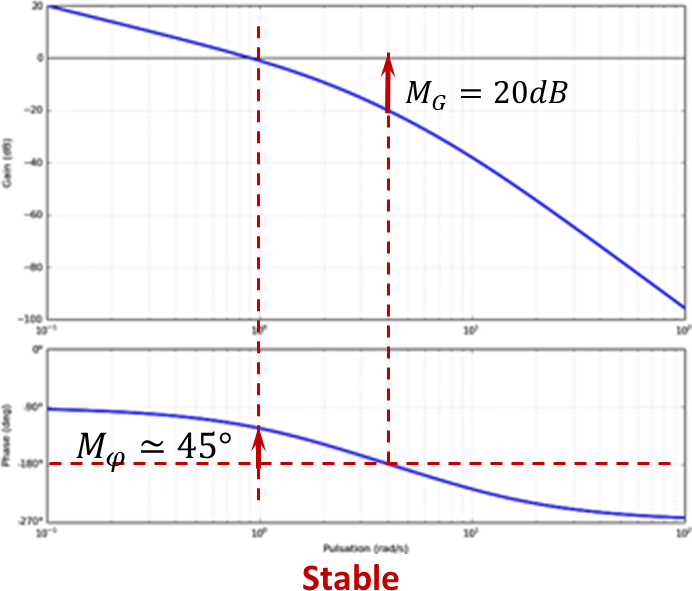
\includegraphics[width=8cm]{im_03_cor}
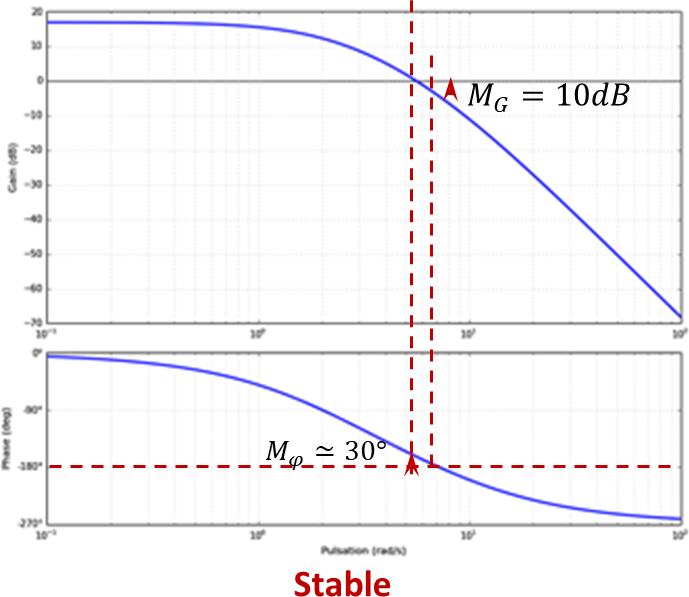
\includegraphics[width=8cm]{im_04_cor}
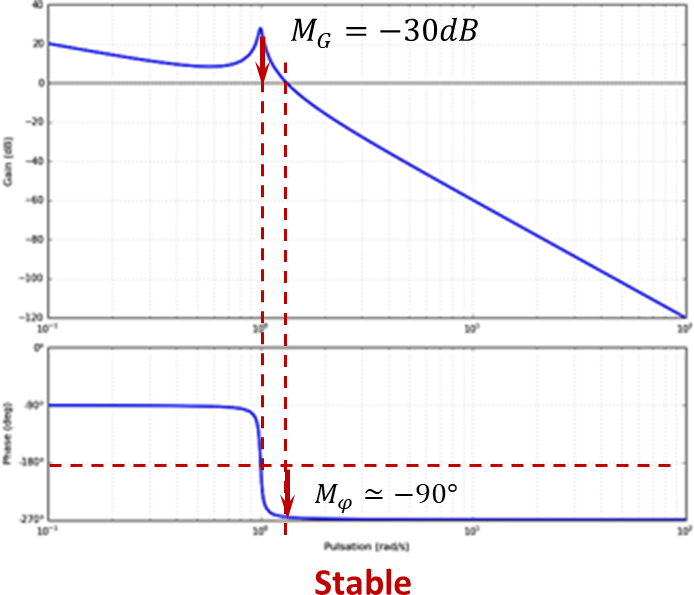
\includegraphics[width=8cm]{im_05_cor}
\end{center}

\else
\begin{minipage}[c]{.48\linewidth}
\begin{center}
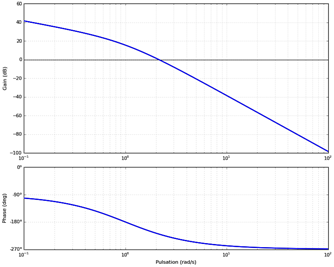
\includegraphics[width=\linewidth]{im_01}
\end{center}
\end{minipage}
\begin{minipage}[c]{.48\linewidth}
\begin{center}
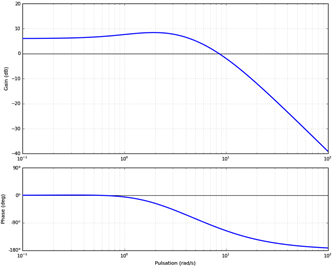
\includegraphics[width=\linewidth]{im_02}
\end{center}
\end{minipage}


\begin{minipage}[c]{.48\linewidth}
\begin{center}
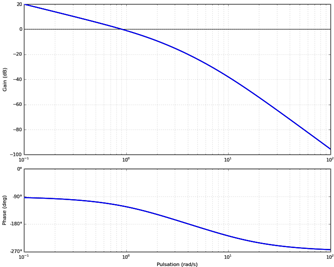
\includegraphics[width=\linewidth]{im_03}
\end{center}
\end{minipage}
\begin{minipage}[c]{.48\linewidth}
\begin{center}
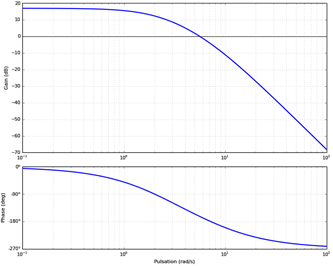
\includegraphics[width=\linewidth]{im_04}
\end{center}
\end{minipage}


\begin{center}
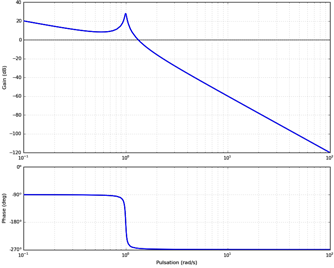
\includegraphics[width=.5\linewidth]{im_05}
\end{center}
\fi



